\section{Countermeasures}
\label{sec:countermeasures}
Authorization mechanism like GoodUSB\cite{tian2015defending} has been proposed as a countermeasure against BadUSB attack. But as mentioned in Section~\ref{sec:badusb} and Section~\ref{sec:experiment}, GoodUSB relies on internal display to request for authorization, which can be hijacked by our \tool. Hence, GoodUSB is indeed a great defense against traditional BadUSB attack but no defense at all for our \tool. Here we discuss some effective countermeasures against \tool.

\textbf{External Hardware Authorization.}
One possible countermeasure is to introduce external hardware completing the authorization process. Contrary to the GoodUSB, USBCheckIn\cite{usbcheckin} adopts a dedicated hardware between the host and device. When a device is plugged in, the authorization will be complete on the dedicated hardware instead of internal display, preventing the host from being hijacked. Though USBCheckIn is a adequate defense against \tool, the external hardware brings additional cost and inconvenience, especially for mobile device.

\textbf{Distrust-by-Default.}
Most security issues of USB protocol is due to its \textit{trust-by-default} policy. \tool also relies on this feature to work. Hence if we reject all \textit{unauthorized} device, \tool and other many USB attacks will fail. It is worth mentioning here that \textit{distrust-by-default} policy is not the same as GoodUSB\cite{tian2015defending}. GoodUSB relies on the \textit{unauthorized} device to complete its own authorization, while in this strict policy, users have to use an \textit{authorized} device. Though \textit{distrust-by-default} policy effectively prevents these attack, this also causes considerable inconvenience for users. For example, when there is no other \textit{authorized} device plugged, it is impossible for user to complete the authorization in the first place. Thus this strict policy is far from optimal in most use cases.

\textbf{Isolated UI Rendering}
During our experiment, we noticed that \tool is actually unable to redirect out the locking screen keyboard from the iPad OS. Instead, the keyboard is only available on the internal display. However, this defense is only enabled on the locking screen keyboard, other virtual keyboard is still vulnerable to our \tool. This mechanism has inspired us to propose a new defense against our \tool called \emph{Isolated UI Rendering}. As illustrated in Figure~\ref{fig:isolated_ui}, we designed two separated UI render driver, one is secure the other is insecure. When an application require to render, it can pass the content along with a tag identifying whether the content is ``sensitive'' or not. If the content is tagged with ``sensitive'', then the OS will only pass it to the secure driver, which only trusts the internal display. On the other hand, if the content is tagged with ``insensitive'', then it will be passed to both secure and insecure driver, rendered on both internal and external display.
\begin{figure}[htbp]
	\centering
	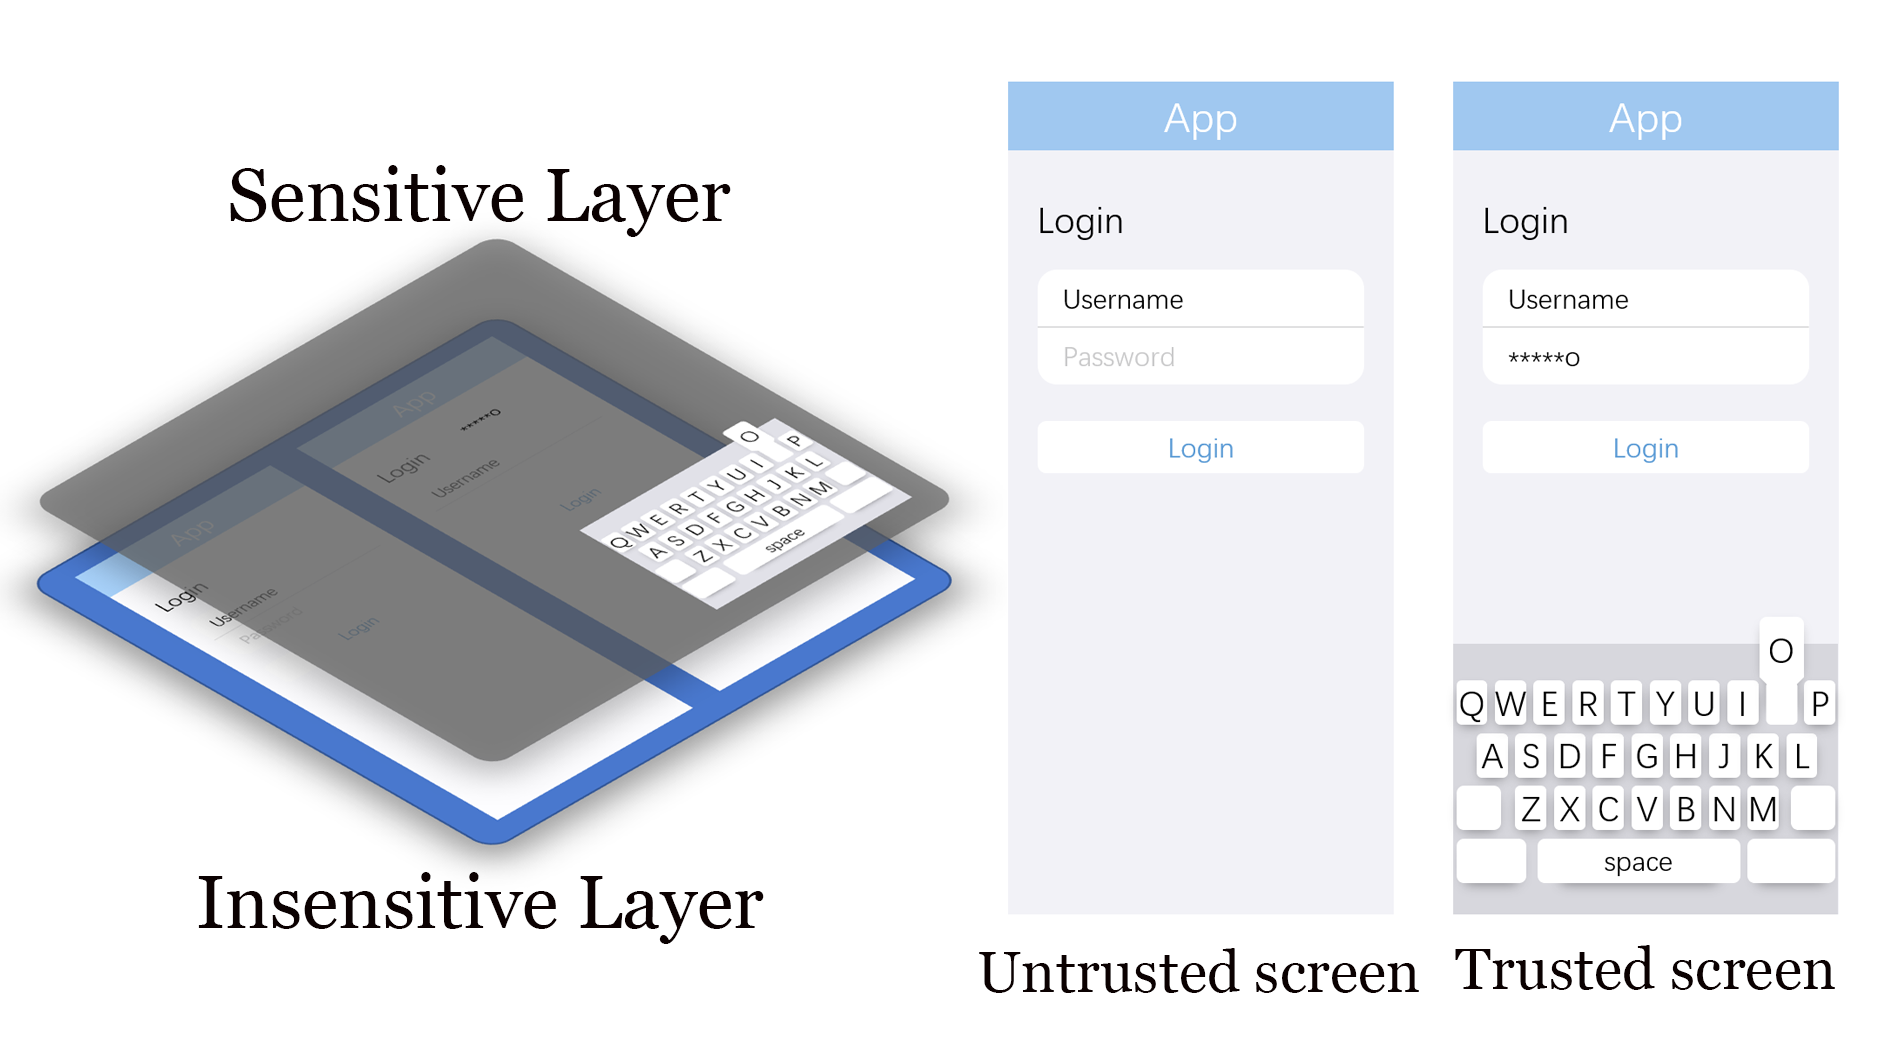
\includegraphics[width=\linewidth]{./Figs/isolated_ui.png}
	\caption{Isolated UI Rendering}\shuqing{Maybe we can increase the font?}
	\label{fig:isolated_ui}
\end{figure}

